\chapter[Sculpting of Liquid Animations]{Sculpting of Liquid Animations}
\label{chap:fluidsculpting}
\Lettrine{D}{ue} to advances in fluid simulation methods over the last two decades, liquid animation has become commonplace in 3D animation productions. 
The animations can be either highly realistic --- for example showing plausible fluid dynamics and interactions with obstacles --- or they can exhibit a more expressive behavior to convey specific artistic intentions. In both cases, it is essential for the artist to be able to control the simulation in order to achieve their goals.

As mentionned in Section~\ref{sec:starSimulationControl}, the simulation control is generally achieved through the careful setting of a large number of parameters such as initial conditions, boundary conditions, viscosity, or external forces. 
We briefly summarize why the tuning of these parameters is particularly difficult.
First, they only offer indirect control over the animation, which makes them quite non-intuitive. 
Second, it is usually not possible to have interactive visual feedback when modifying the parameters, due to the high computational cost of 
liquid simulation.
Third, the inherently non-linear nature of fluid behavior makes it difficult to transfer parameter values from a low to a high resolution simulation. 
In consequence, achieving a desired effect requires a tedious trial-and-error loop, where computation is restarted multiple times from scratch with different parameters. 
In many cases, this process does not allow tight control over a sequence of waves and splashes with specific magnitudes or shapes and occurring in a specific order. 

In this chapter, we attempt a significanly different approach.
Instead of controlling a simulation, we propose an interactive sculpting system for seamlessly editing pre-computed animations of liquid, without the need for any re-simulation. 
Our system is based on a copy/edit/paste approach:
The user can efficiently select consistent and visually important space-time parts of a liquid animation, such as moving waves or droplets, that we call \emph{space-time features};
Once selected, these space-time features can be copied and edited in both space and time in order to change their size, orientation, trajectory or speed;
Finally, the edited space-time features can be pasted back into any destination animation at a specific position and time set by the user.

Using our tools, the user can edit and progressively refine any input simulation result, possibly using a library of pre-computed space-time features extracted from other animations. 
In contrast to the trial-and-error loop usually required to edit animation results through the tuning of indirect simulation parameters, our method gives the user full control over the edited space-time behaviors. 

To enable the use of arbitrary liquid animations computed using varying simulation techniques, we based our editing framework on generic inputs; 
our method allows input mesh sequences without point-wise correspondences between frames, and with arbitrary changes of topological genus between two consecutive time steps.
Also, we focused on three requirements to make our method useful in realistic cases.
First, the selection of the effect in the original simulation must be as simple and straightforward for the user as possible. 
Therefore, once space-time features have been computed, the user can select them using a simple click on the surface.
Secondly, pasting the selected effect onto the final animation should be handled automatically, with seamless adaptation of the pasted fluid effect to the destination surface. 
Finally, the pipeline of selection, copy, edit, and paste steps should be computed efficiently in order to enable interactive user feedback. 
\paragraph*{}
The key contributions of our work are as follows:
\begin{itemize}
    \item A semi-automatic method to tag salient regions in a liquid animation.
    \item An algorithm that extracts coherent \emph{space-time features} from a mesh sequence with tagged vertices.
    \item A \emph{space-time feature} representation independent from the original animation.
    \item A set of editing operations that allow the extraction, manipulation, and insertion of \emph{space-time features} into an animation.
\end{itemize}
The remainder of this chapter is organized as follows:
Section~\ref{sec:overview} presents our solution to this problem;
Section~\ref{sec:extraction} explains how \emph{space-time features} are computed; 
Section~\ref{sec:representation} deals with the \emph{space-time features} representation; 
Section~\ref{sec:manipulation} details the tools we offer for manipulating \emph{space-time features}; 
Section~\ref{sec:fluidsculpting:results} shows results obtained with our method; 
Section~\ref{sec:fluidsculpting:discussion} draws the limits of our approach and gives some perspectives on future work.
\paragraph*{}
The works described in this chapter have been submitted to the conference \emph{MIG 2016}. We describe our method and results in the video here: \url{https://www.dropbox.com/s/0cob2nuztdimjol/fluidSculpting_MIG2016.mp4?dl=0}.

\section{Overview of the method}\label{sec:overview}
As mentioned above, this chapter focuses on editing liquid animations.
To be independent from the simulation method, we take as input a sequence of meshes without any correspondences between the mesh vertices from one frame to another. 
Due to the arbitrary topology of the meshes and to the temporal coherence to be maintained for numerous geometric details, editing each frame with a shape modeling tool would represent a tremendous amount of work.
Instead, we propose to manipulate a higher level representation of the liquid animation that we call \emph{space-time features}. A space time feature is a sub-part of the animation, i.e. a sequence of sub-parts of the liquid surface. 

Our editing pipeline generalizes standard sculpting tools~\cite{Ferley2000} based on cut/copy/edit/paste operations.
It is made of three steps which are illustrated in Figure~\ref{fig:overview}. 
\begin{figure}[!h]
	\centering
	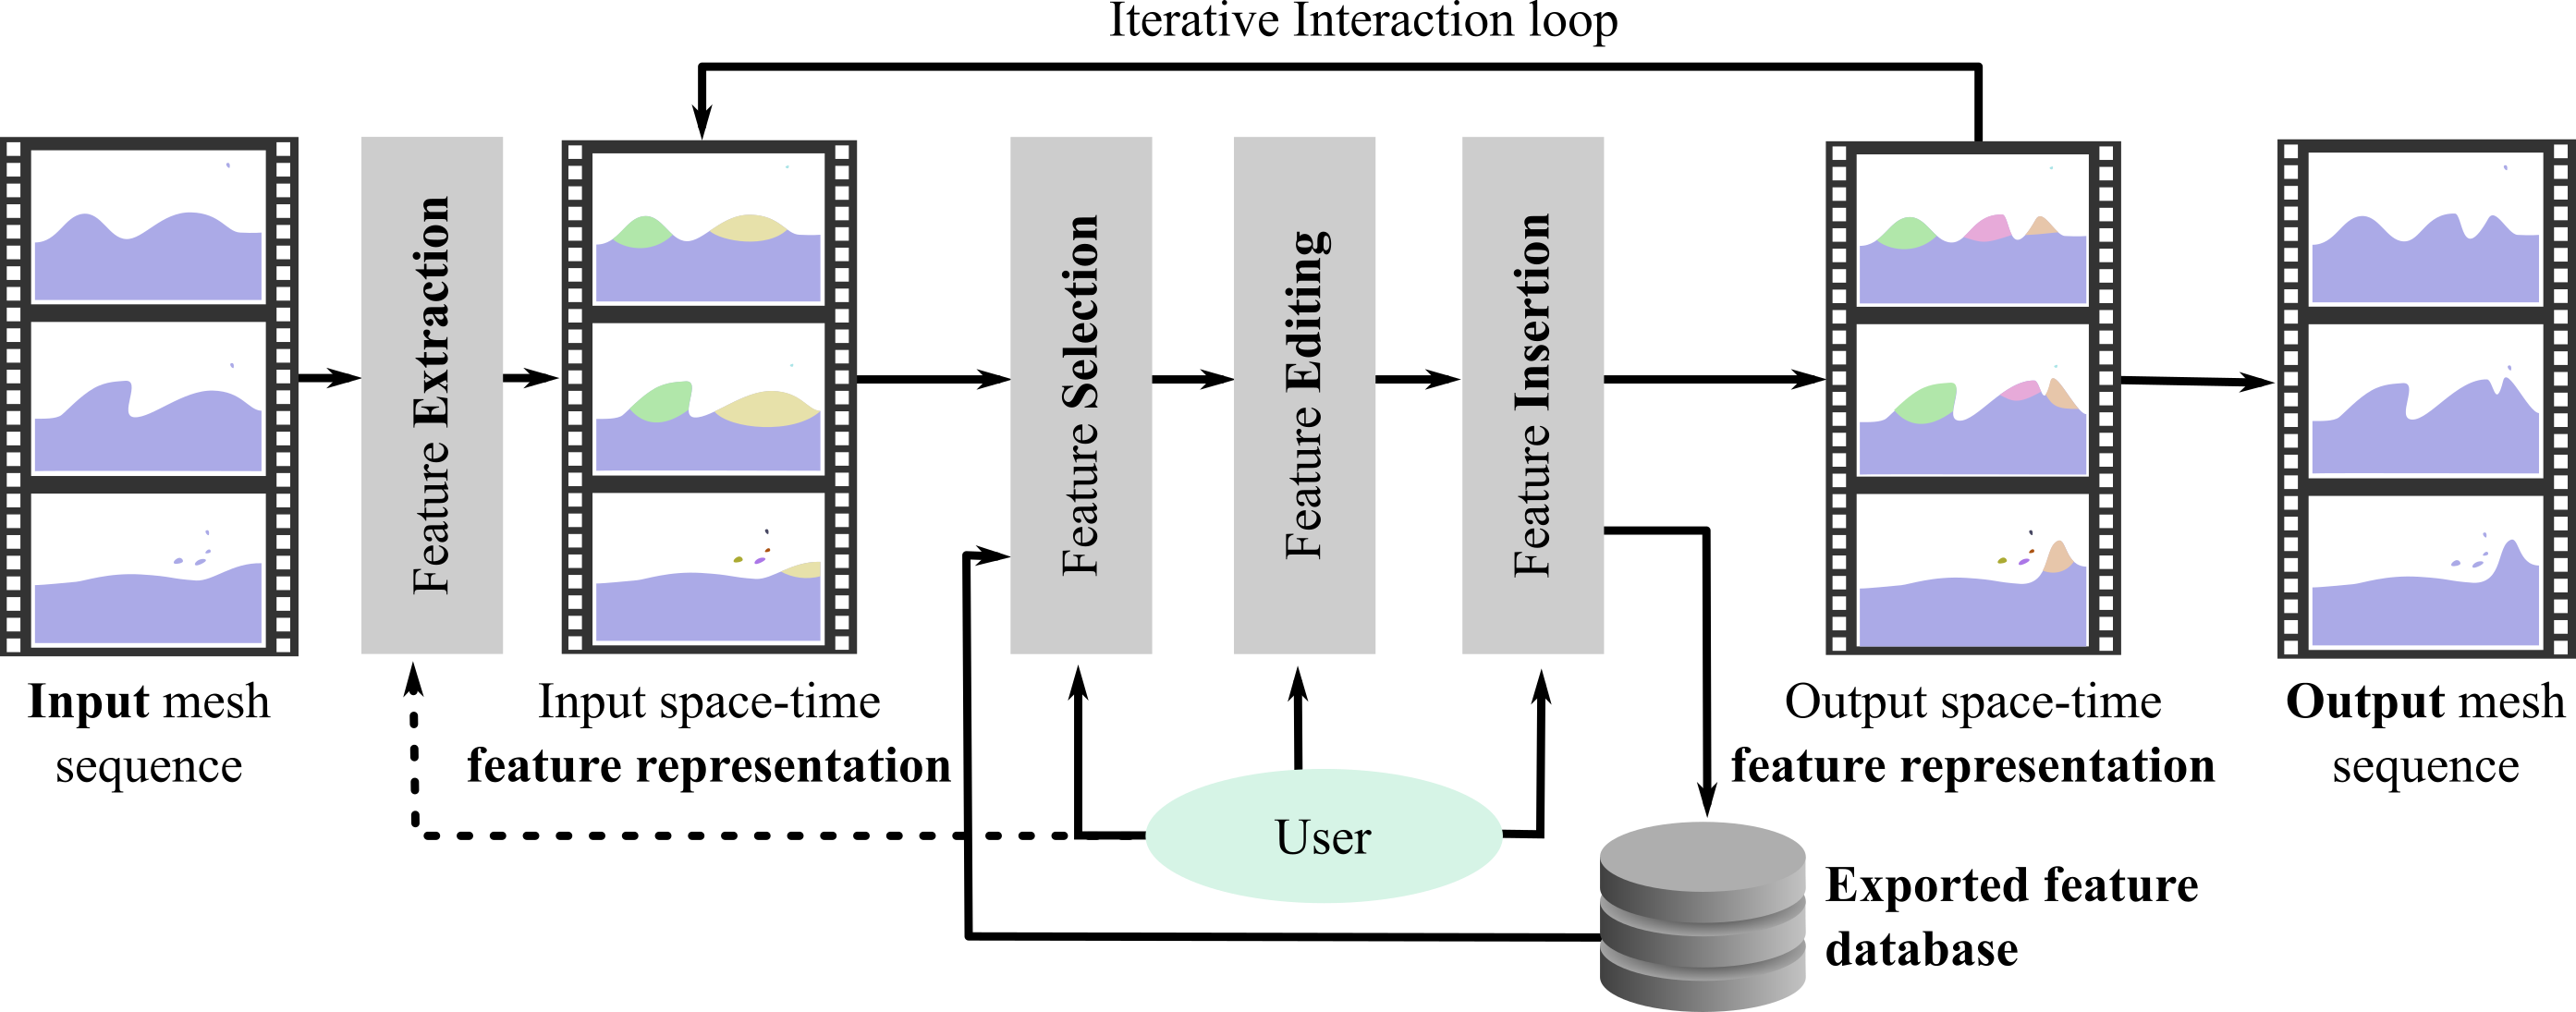
\includegraphics[width=\linewidth]{images/fluidsculpting-mig2016/overview_2.png}
	\caption[Fluid sculpting: Overview]{
		Pipeline of our method: 
		An input fluid animation is given as a mesh sequence. 
		It is pre-processed into a higher-level space-time feature representation. 
		This representation allows the user to iteratively select features from the animation and edit them before inserting them back to the animation. 
		Alternatively, features can be saved and re-imported in this animation or a different one. }
	\label{fig:overview}
\end{figure}

The first step extracts space-time features from the animation. As these features represent regions that deform over time, it would be too tedious for a user to define them by hand. We propose a semi-automatic method to detect salient regions in a liquid animation from which space-time features will be automatically computed. 
The user can then easily select them using picking: a click at a specific location at a given frame in time results in the automatic selection of the associated feature with its full range in space and time.
The second step computes representations of the selected space-time features that are independent from the input animation.
They enable space-time features to be transferred from one animation to another. 
Finally, the last step consists of editing the space-time features and pasting them back into an animation.


\section{Feature extraction}
\label{sec:extraction}
 In the feature extraction step, our method defines the space-time features that the user would like to manipulate. 
This process is divided into three steps, as described in Figure~\ref{fig:feature_extraction}: detection, segmentation, and aggregation. 
While detection is semi-automatic (it is interleaved with user interaction to define customized regions of interest throughout the animation), segmentation and aggregation are fully automatic.
 \begin{figure}[!h]
 	\centering
 	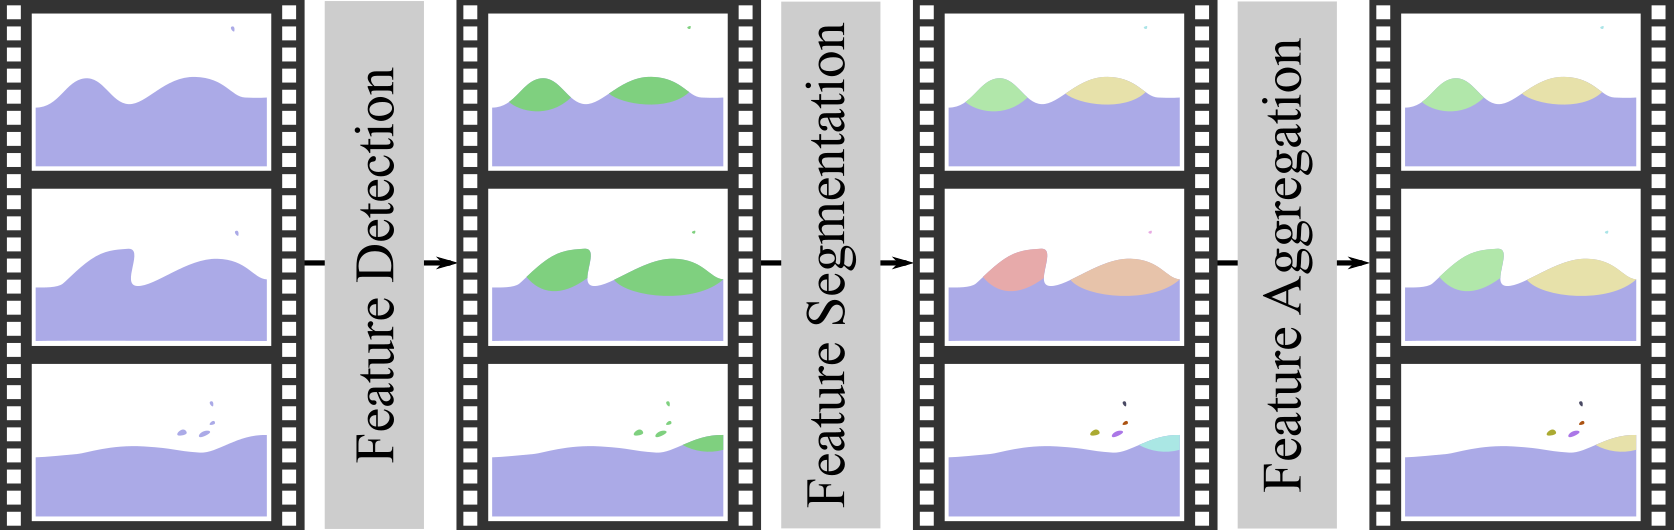
\includegraphics[width=\linewidth]{images/fluidsculpting-mig2016/feature_extraction_2.png}
 	\caption[Fluid sculpting: Feature extraction]{Feature extraction process, from left to right: an initial mesh sequence representing a fluid animation is subjected to a feature detection process, followed by a segmentation step, which results in a frame feature representation. 
 		A final aggregation step allows to build a temporally coherent feature structure.}
 	\label{fig:feature_extraction}
 \end{figure}

\paragraph{Notation}
The input of our method is a mesh sequence over the time steps $t$ that we note $M = (M^t)$, where $M^t$ is a manifold triangular mesh.
We note $T(.)$ the temporal length (i.e. the number of frames) and $L(.)$ the characteristic spatial length of any space-time sequence (mesh sequence or feature).
Given a triangular mesh $X$, we call $N_X$ the set of its vertices and $P_X$ the set of its faces.
A vertex can carry attributes. We note $A(n,X)$ the value of the attribute $A$ at the vertex $n$ of the mesh $X$. In the following, we will note $pos(n,X)$, $norm(n,X)$, and $curv(n,X)$ for positions, normal, and curvature respectively.
$\Delta_{A}(n,X)$ designates the Laplace-Beltrami operator applied to the attribute $A$ at vertex $n$ of the mesh $X$.
%A comprehensive list of notations can be found in Appendix~\ref{sec:notations}.

\subsection{Detection}\label{sec:features:detection}

The detection phase aims at defining a sequence of regions of interest $R = (R^t)$ on $M$.
A region $R^t$ is represented as a set of vertices of $M^t$; we call this structure a \emph{mesh part}. 

To let the user easily and intuitively define $R$, we propose a semi-automatic tool.
This tool is based on two key components that we describe in detail below: 
curvature analysis and topological filtering.
Combined together they let the user define $R$ in a coarse-to-fine manner: 
First, curvature analysis is used to automatically detect salient features at each frame and initialize $R$. 
Then, topological filtering allows to interactively adjust $R$. 
We also added a painting tool that allows the user to fine-tune each $R^t$ if needed by locally removing or adding vertices from $R$ by clicking.

\paragraph*{Multi-resolution curvature analysis.}
We chose a curvature criteria to extract features as it is a natural asset for detecting waves and ripples in liquid animations. Moreover, the intimate relationship between surface curvature and liquid surface dynamics had already led previous work to use curvature as a tool to enrich liquid simulations, for example with splashes~\cite{Takahashi2003}, foam~\cite{Ihmsen2012} and textures~\cite{Narain2007}.

Curvature is computed at each vertex $n$ of the animation meshes $M^t$ using the following formula:
\begin{equation}
curv(n,M^t) = norm(n,M^t) \cdot \Delta_{pos}(n,M^t)
\end{equation}
Vertices are colored with respect to their curvature magnitude, enabling the user to interactively observe the curved regions and their deformations on the fluid surface while playing the animation (see Figure~\ref{fig:nonSmoothedCurvature}). 
Then we provide two sliders that the user can interactively tune to filter the curvature and select meaningful regions.
These sliders represent:
\begin{itemize}
\item A number of iterations $\beta$ of Laplacian diffusion on the curvature values.
We define the $i$-th iteration of the Laplacian curvature diffusion as:
\begin{equation}
    curv^{i+1}(n,M^t) = curv^i(n,M^t) - \lambda . \Delta_{curv^i}(n,M^t)
\end{equation}
with $curv^0(n,M^t) = curv(n,M^t)$ and $i \in \left[0,\beta\right]$.
In our experiment, we used $\lambda=1$ as a diffusion factor.
Laplacian diffusion of the computed curvature values is used to decrease the spatial frequency of the curvature function over the surface.
This allows the user to select broader regions in an efficient way without actually smoothing the geometric details on the mesh (see Figure~\ref{fig:smoothedCurvature}). 
\item A threshold $\gamma$ on the curvature of $R$. All the vertices whose curvature is above $\gamma$ are added to $R$. This allows the user to control the extent of $R$ (see Figure~\ref{fig:curvatureThreshold}). 

In the end, we can mathematically define a region of interest for a frame $t$ as:
\begin{equation}
 R^t = \{ n\in N_{M^t} \vert curv^{\beta}(n,M^t) > \gamma \}
\end{equation}
\end{itemize}

\begin{figure}[t]
\centering
    \begin{subfigure}[b]{0.45\linewidth}
    \centering
    \includegraphics[width=\textwidth]{images/fluidsculpting-mig2016/nonSmoothedCurvature.eps}
    \caption{\label{fig:nonSmoothedCurvature}Mean curvature}
    \end{subfigure}
    \hspace{0.1cm}
    \begin{subfigure}[b]{0.45\linewidth}
    \centering
    \includegraphics[width=\textwidth]{images/fluidsculpting-mig2016/smoothedCurvature.eps}
    \caption{\label{fig:smoothedCurvature}Smoothed curvature}
    \end{subfigure}
    \begin{subfigure}[b]{0.45\linewidth}
    \centering
    \includegraphics[width=\textwidth]{images/fluidsculpting-mig2016/curvatureThreshold.eps}
    \caption{\label{fig:curvatureThreshold}Curvature thresholding}
    \end{subfigure}
    \hspace{0.1cm}
    \begin{subfigure}[b]{0.45\linewidth}
    \centering
    \includegraphics[width=\textwidth]{images/fluidsculpting-mig2016/featureZone.eps}
    \caption{\label{fig:featureZone}Topological closure}
    \end{subfigure}
    \caption[Fluid sculpting: Feature detection]{
\label{fig:curvature_analysis}
Curvature analysis-based feature detection.
}
\end{figure}

\paragraph*{Topological filtering.}
In many cases, curvature-based selection is not sufficient to extract meaningful animation features. 
For instance, in Figure~\ref{fig:curvatureThreshold}, the user might want to select the whole crown splash and not only its contour as it has been done with the curvature analysis tool. 
To remedy these issues, we extend mathematical morphological operators (MMOs) to polygonal meshes.
They allow the user to interactively and easily refine the regions of interest detected by the curvature analysis.

We propose two main tools:
\begin{itemize}
 \item \emph{Erosion} for disconnecting, reducing or removing parts of $R$.
 \item \emph{Dilatation} for connecting and enlarging parts of $R$.
\end{itemize}
Both tools can be combined for performing \emph{openings} and \emph{closures} of $R$.
In practice, these tools were particularly useful for selecting regions such as the interior part of the circular wave in Figure~\ref{fig:featureZone}, achieved with a closure.
For a detail overview of MMOs, we refer the reader to the work of Serra~\cite{Serra1986}.
%and to Appendix~\ref{sec:mesh_part}.

\subsection{Segmentation}\label{sec:features:segmentation}
Once $R$ has been computed, the segmentation step decomposes each $R^t$ into connected components $(C_k^t)_{k,t}$, where $k$ is the index of the component. Mathematically, a region of interest for a frame $t$ can be defined as the disjoint union of its connected components:
\begin{equation}
 R^t = \bigsqcup_k C_k^t \text{~~} \vert \text{~~} \forall t \in [0, T(M)-1]
\end{equation}
The decomposition is computed using the straightforward breadth-first search on each frame in parallel. 
We call each $C_{k}^{t}$ a \emph{frame feature}.

\subsection{Aggregation}\label{sec:features:aggregation}
Finally, the aggregation step extracts temporally coherent sequences of \emph{frame features} that we call \emph{space-time features}. 
The process is divided into two steps as illustrated in Figure~\ref{fig:aggregation}.
First, we build a graph of all possible \emph{frame feature} connections, and then we compute a vertex-disjoint path cover of that graph. Temporal coherency of the resulting paths is enforced by minimizing a geometric matching cost described below. We call the resulting paths \emph{space-time features}.
\begin{figure}[!h]
	\centering
	\begin{subfigure}[b]{0.48\linewidth}
		\centering
		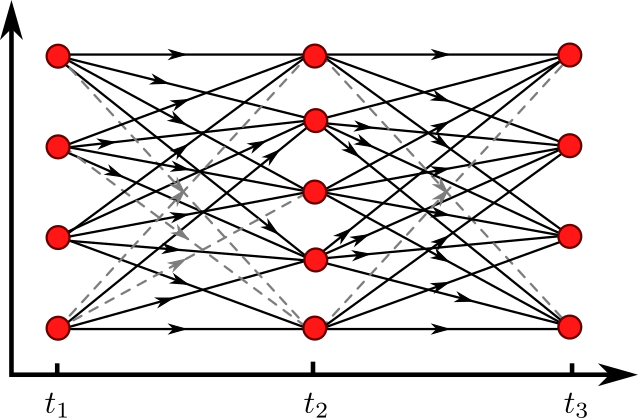
\includegraphics[width=\textwidth]{images/fluidsculpting-mig2016/dag_features.png}
		\caption{\label{fig:dagFeatures}Initial DAG}
	\end{subfigure}
	\hspace{0.1cm}
	\begin{subfigure}[b]{0.48\linewidth}
		\centering
		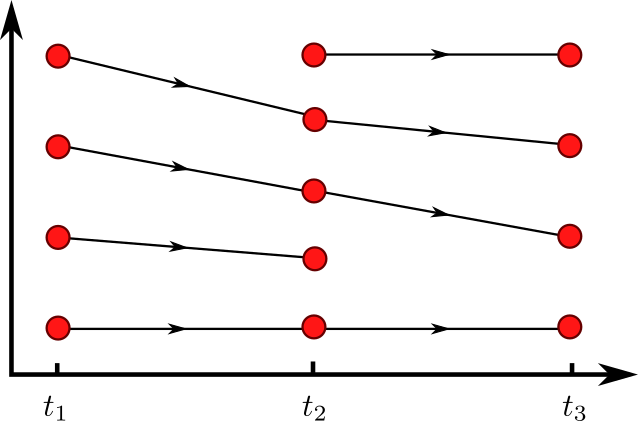
\includegraphics[width=\textwidth]{images/fluidsculpting-mig2016/aggregation_step2.png}
		\caption{\label{fig:aggregatedFeatures}Vertex-disjoint path cover}
	\end{subfigure}
	\caption[Fluid sculpting: Feature aggregation]{
		Left: Frame features (red dots) are assembled into a directed acyclic graph as described in Section~\ref{sec:features:aggregation}.
		Each edge of the graph carries a cost computed with Equation~(\ref{eq:costfunction}). 
		Edges whose cost is over a user-defined threshold (gray dashed lines) are discarded.
		Right: a vertex-disjoint minimum-cost path cover has been computed based on Algorithm~(\ref{alg:aggregation}). 
		The extracted paths represent space-time features.}
	\label{fig:aggregation}
\end{figure}

\paragraph*{Graph construction.}

We build a directed acyclic graph $G = (V_G, E_G) $ representing the possible connections between frame features (see figure~\ref{fig:dagFeatures}).
The set of nodes $V_{G}$ is made of the frame features $\left(C_{k}^{t}\right)_{k,t}$ while the set of edges $E_{G}$ is made of oriented edges $e_{ij}$ linking each pair of consecutive frame features $C_{i}^{t}$ and $C_{j}^{t+1}$.

\paragraph{Edge cost computation}

For every edge $e_{ij}\in E_{G}$, we compute a cost measure \(\omega_{ij}\). This measure relates to the geometrical matching between its two endpoints $v_{i}$ and $v_{j}$.
We divided \(\omega_{ij}\) into three terms:
\begin{itemize}
    \item $d_{ij}$: The distance between the centers of mass of $v_{i}$ and $v_{j}$.
    \item $s_{ij}$: The difference of the surface area between $v_{i}$ and $v_{j}$.
    \item $v_{ij}$: The difference of volume between $v_{i}$ and $v_{j}$. $v_{ij}$ is computed only if both $v_{i}$ and $v_{j}$ are closed.
\end{itemize}
The edge cost $\omega_{ij}$ is a weighted sum of these terms, normalized by the appropriate power of $l=L(M)$, the characteristic size of the bounding box of $M$:
\begin{equation}
\label{eq:costfunction}
\displaystyle \omega_{ij} = 
\omega_{d}\, \left(\frac{d_{ij}}{l  }\right)^2 +
\omega_{s}\, \left(\frac{s_{ij}}{l^2}\right)^2 + 
\omega_{v}\, \left(\frac{v_{ij}}{l^3}\right)^2
\end{equation}
For all the examples of this chapter we used $\left( \omega_{d}, \omega_{s}, \omega_{v} \right)$ = $\left(0.6,0.2,0.2\right)$. We chose to favor the closeness between frame features and consider difference of surface and volume equally. After the cost computation, we discard edges whose cost is below a threshold $\epsilon$ that we set to $0.3 \times l$ in our examples. Higher thresholds lead to fewer edges in the graph and more disconnected paths.

\paragraph*{Vertex-disjoint path cover computation.}

To the authors' knowledge, there is no standard algorithm for computing minimum weight vertex-disjoint path cover. 
We propose an algorithm based on Kruskal's algorithm for computing minimum spanning trees~\cite{kruskal1956shortest}:
All vertices are first copied from the input graph to the output one;
edges of the input graph are considered in ascending order of cost and added to the output graph if they satisfy a given topological condition.
In Kruskal's algorithm, the condition is that the edge does not form a cycle in the output graph.
In ours, the condition is that both of its endpoint vertices have strictly fewer than two neighbors.
This allows us to ensure that the resulting path cover will be vertex-disjoint. 

We detail our vertex-disjoint path cover process in Algorithm~\ref{alg:aggregation} using the following notation:
\begin{itemize}
  \item $G$, $V$, and $E$ represents respectively a graph, a set of vertices, and a set of edges;
  \item $in$ and $out$ subscripts refer to input and output elements;
  \item $v^e_0$ and $v^e_1$ refer to the endpoints of edge $e$ in both $G_{in}$ and $G_{out}$ (since $V_{in} = V_{out}$);
  \item $deg(v)$ is the degree of vertex $v$ in $G_{out}$;
  \item $sort(E)$ is the in-place sort of the edges of $E$ in the ascending cost order.
\end{itemize}

\begin{algorithm}[H]
    \caption[Fluid sculpting: Aggregation]{~~Vertex-disjoint path cover computation} 
\label{alg:aggregation}
\begin{algorithmic}
\State $ G_{in}  = ( V_{in},  E_{in}  ) $ 
\State $ G_{out} = ( V_{out}, E_{out} ) $ 
\State $ V_{out} = V_{in}$ 
\State $ E_{out} = \varnothing $
\State $ sort(E_{in}) $
\ForAll{ $ e \in E_{in} $ }
  \If { $deg(v^e_0) < 2$ \textbf{and} $deg(v^e_1) < 2$}
  	\State $E_{out} \gets e$
  \EndIf
\EndFor
\end{algorithmic}
\end{algorithm} 
At the end of this algorithm, the graph $G_{out}$ consists of all frame-features $V_{out}$ connected by inter-frame links $E_{out}$.
$E_{out}$ represents independent paths, as illustrated in Figure~\ref{fig:aggregatedFeatures}, which are optimal in the sense that the algorithm greedily minimizes our edge cost metric. 
These paths describe the \emph{space-time features}. 

\section{Feature representation}
\label{sec:representation}
Space-time features can be seen as a simple set of vertices belonging to $M$.
This representation is, however, inconvenient for direct manipulation as it strongly depends on the input animation and therefore cannot be transferred from one animation to another. 
To be able to copy, edit and paste space-time features in different animations, we propose to build a representation of a space-time feature which is independent from $M$.

In the remainder of this chapter, we will note a space-time feature representation $F_{i} = \left( F_{i}^{t} \right)_{t^{s}\left(F_{i}\right) \leq t \leq t^{e}\left(F_{i}\right)}$ where $t^{s/e}(F_{i})$ are the starting/ending frame index of $F_{i}$ and $F_{i}^{t}$ is the frame feature representation of $F_{i}$ at the frame $t$. 
Also, we denote by $S(F_{i}^{t})$ the mesh part of $M^{t}$ corresponding to $F_{i}^{t}$.

We distinguish two representations depending on whether the frame feature has boundaries or not (see Figure~\ref{fig:feature_representation}). 
\begin{figure}[h!]
	\centering
	\label{fig:featureRepresentation}
	\begin{subfigure}[b]{0.46\linewidth}
		\centering
		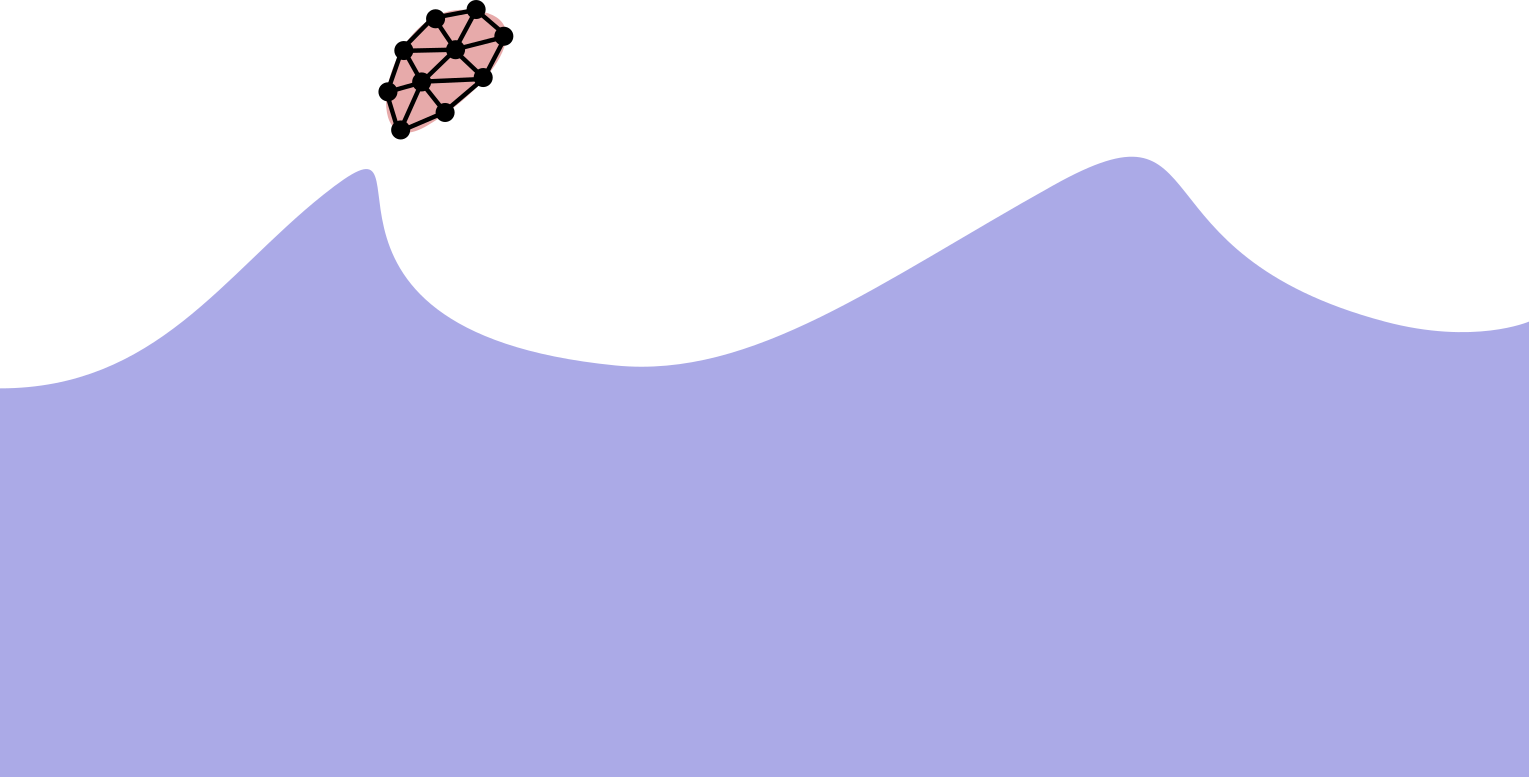
\includegraphics[width=\textwidth]{images/fluidsculpting-mig2016/isolatedFeature.png}
		\caption{\label{fig:feature_representation:mesh}Mesh representation}
	\end{subfigure}
	\hspace{0.1cm}
	\begin{subfigure}[b]{0.46\linewidth}
		\centering
		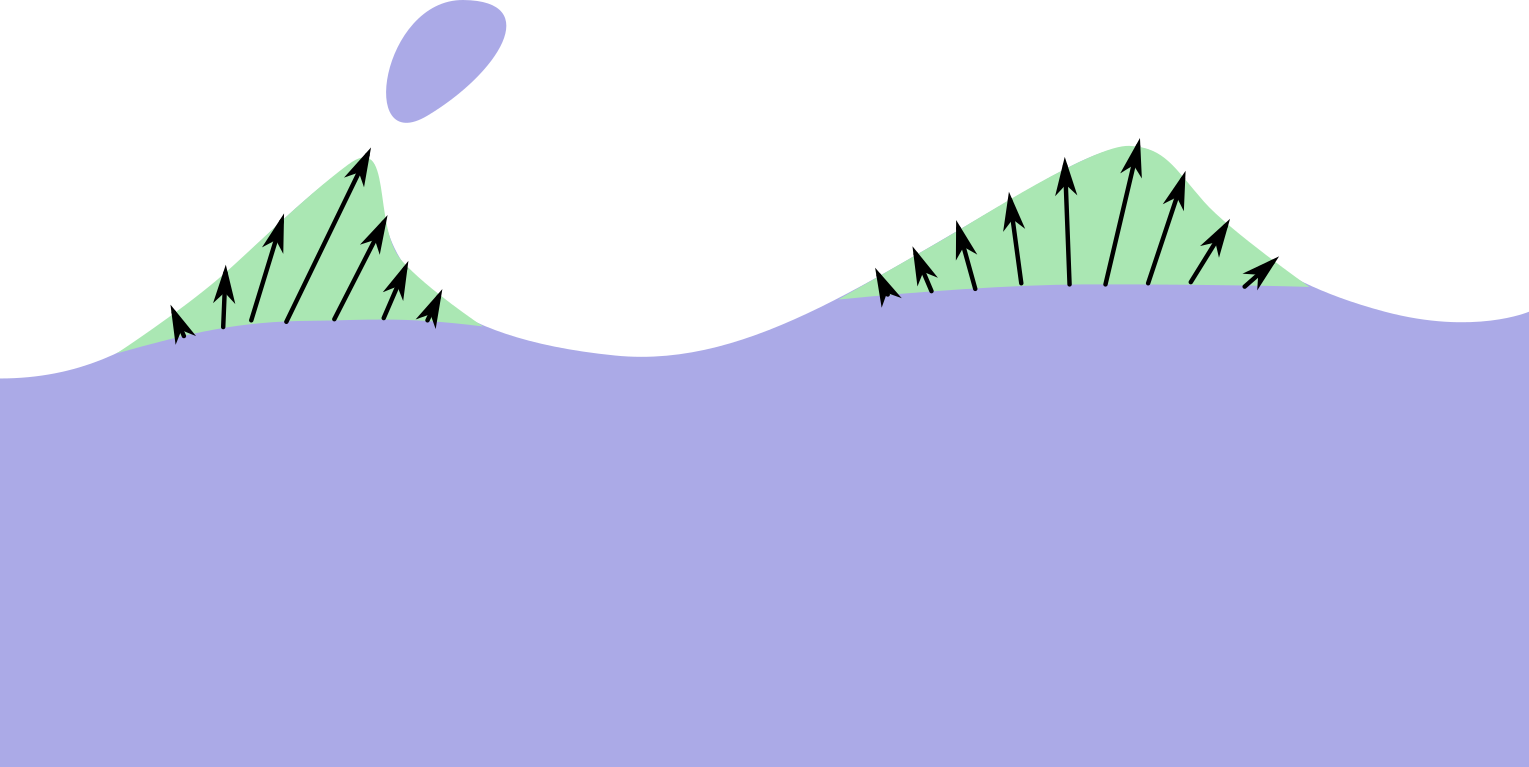
\includegraphics[width=\textwidth]{images/fluidsculpting-mig2016/detailFeature.png}
		\caption{\label{fig:feature_representation:displacement}Differential representation}
	\end{subfigure}
	\caption[Fluid sculpting: Feature representation]{
		Depending on whether the frame feature has closed boundaries or not, it is stored either as a mesh (left) or as a displacement field (right).}
	\label{fig:feature_representation}
\end{figure}

In the first case, we use a \emph{mesh representation}, noted $M(F^t_i)$ and composed of a simple $3$D mesh. 
It is used to represent a connected component of the liquid, such as droplet or a larger body of water.
In the second case, we use a \emph{differential representation}, noted $(\tau_d(F^t_i), \tau_n(F^t_i))$, and composed of a pair of textures representing a displacement map and a normal map.
It is used for frame features representing a local sub-part of a larger body of water, such as a single wave on the surface of an ocean.
A space-time feature can be composed of frame features from both categories.
A typical case of mixed representation is an isolated drop falling into a larger body of water and becoming a detail of this larger surface.

In the following of this section, we detail the computation of both representations and how they can be inserted back into a different animation. This will be useful later for copying and pasting features.
\begin{figure}[!h]
	\centering
	\begin{subfigure}[b]{0.48\linewidth}
		\centering
		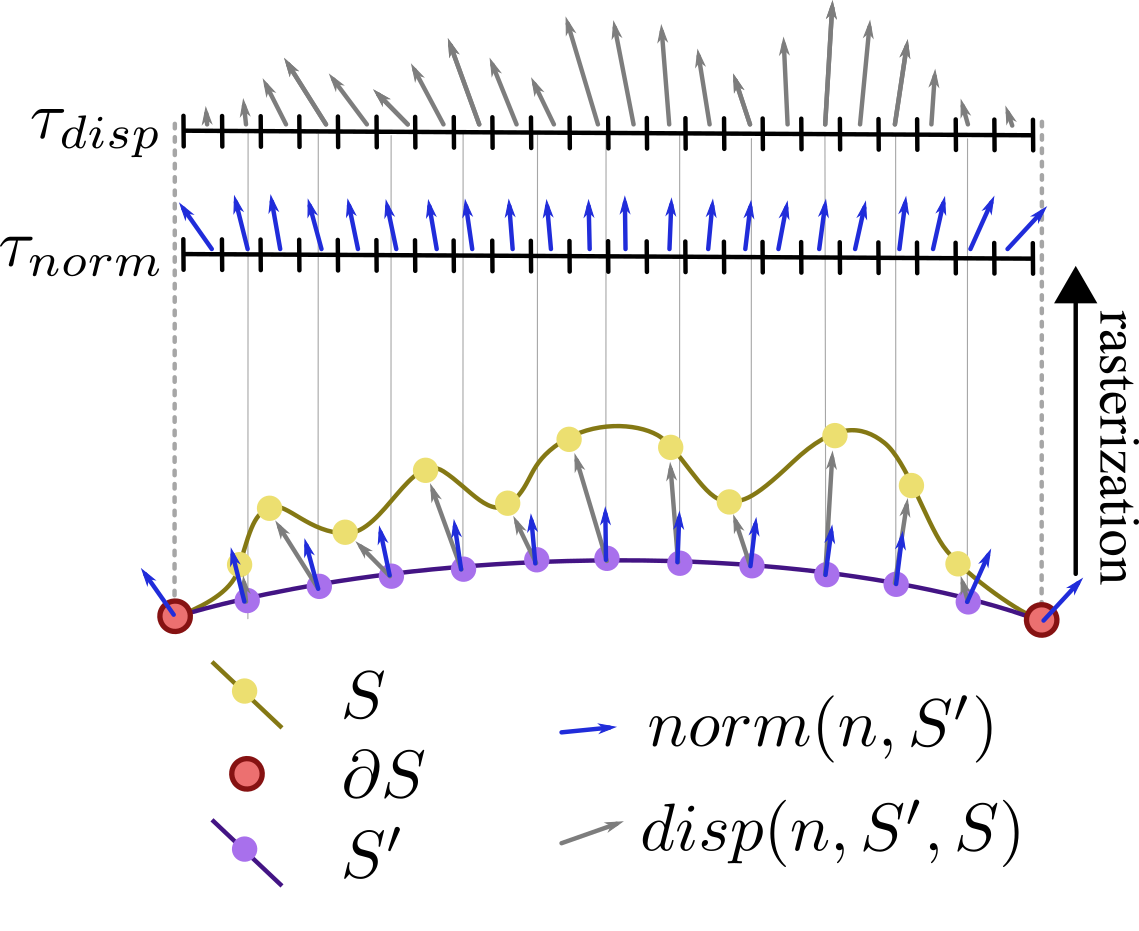
\includegraphics[width=\textwidth]{images/fluidsculpting-mig2016/displacement_copy_2.png}
		\caption{\label{fig:displacement:copy}Copying}
	\end{subfigure}
	\hspace{0.1cm}
	\begin{subfigure}[b]{0.48\linewidth}
		\centering
		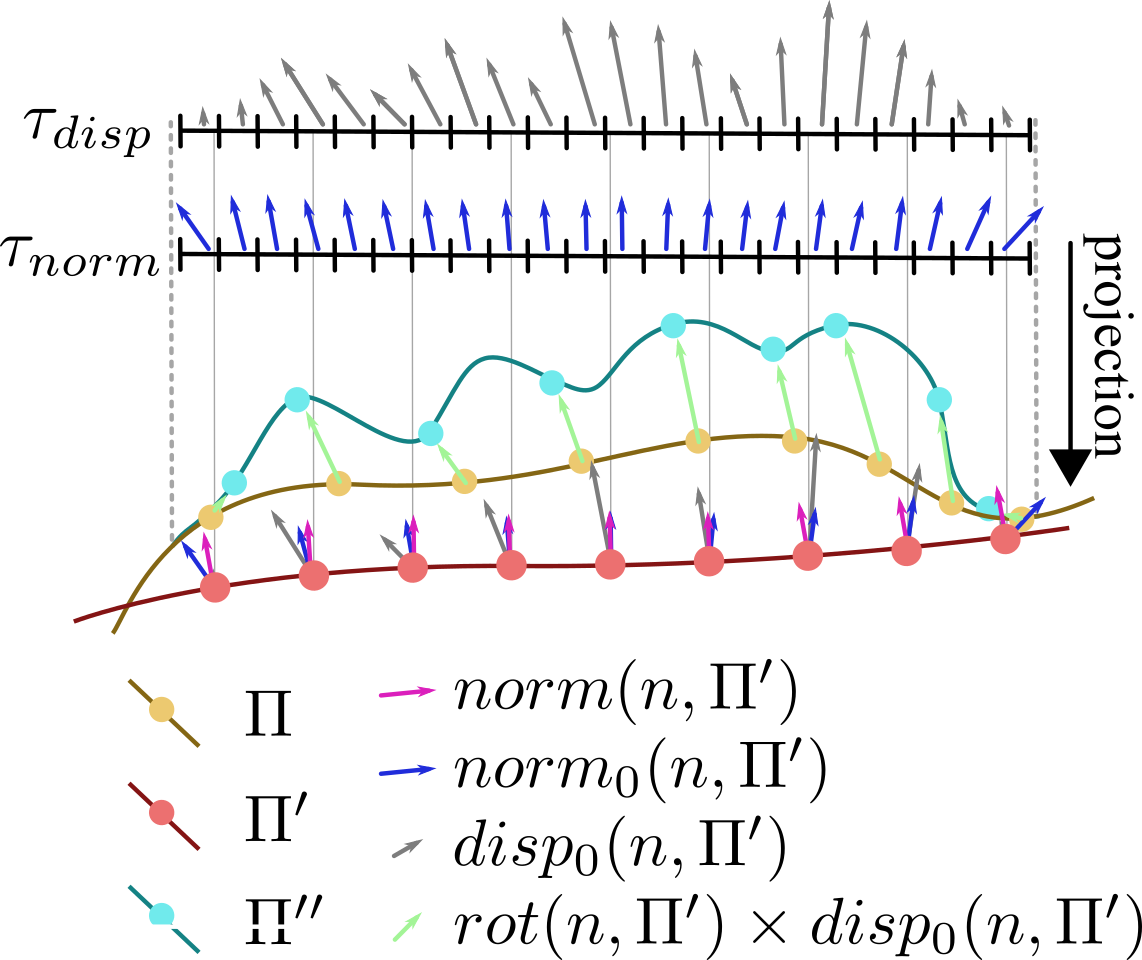
\includegraphics[width=\textwidth]{images/fluidsculpting-mig2016/displacement_paste_2.png}
		\caption{\label{fig:displacement:insertion}Pasting}
	\end{subfigure}
	\caption[Fluid sculpting: Copy/Paste]{
		Left: The displacement representation of a mesh part $S$ is built from the sampling of the displacement field transporting $S'$ toward $S$, and the normal field of $S'$.
		Right: This representation can be inserted back into a mesh part $\Pi$ by projecting a displacement and a normal on vertices of $\Pi'$. 
		The difference of normals between $S'$ and $\Pi'$ is used for orienting the displacements, which are in turn used for generating the deformed surface $\Pi''$.
	}
	\label{fig:displacement}
\end{figure}
\subsection{Computation}
\label{sec:representation:computation}

Building the mesh representation of a frame feature $F^t_i$ simply consists of transforming $S(F^t_i)$ into an independent mesh $M(F^t_i)$.

Building the differential representation of a frame feature is slightly more complex.
The process is described in Figure~\ref{fig:displacement:copy}), and consists of three steps:
Starting from the initial frame feature surface $S(F^t_i)$ we compute a smooth version $S'(F^t_i)$ using Laplacian smoothing on the inner part of the surface $S(F^t_i) \setminus \partial S(F^t_i)$.
We note $pos(n, S)$ the position of vertex $n$ on surface $S$; note that $S(F^t_i)$ and $S'(F^t_i)$ describes the same vertices, but with different positions.
Then we compute the displacement of each vertex $n \in N$ from $S'(F^t_i)$ to $S(F^t_i)$:
\begin{equation}
    disp(n,S'(F^t_i), S(F^t_i) ) = pos(n, S(F^t_i)) - pos(n, S'(F^t_i))
\end{equation}
Finally, we map for every vertex $n$, $disp(n,S'(F^t_i), S(F^t_i))$ onto $S'(F^t_i)$, and sample the linearly interpolated values into the texture $\tau_d(F^t_i)$.
We similarly sample the normals of $S'(F^t_i)$ into $\tau_n(F^t_i)$.
The samplings are performed on the GPU using the standard off-screen rasterization pipeline.

\subsection{Insertion}
\label{sec:representation:insertion}

Mesh representations are trivially inserted by copying $M(F^{t'}_i)$ into $M^t$.

To insert a feature representation $(\tau_d(F^{t'}_i), \tau_n(F^{t'}_i))$ into $M^t$ at location $p$, we first need to identify the part $\Pi \subset M^t$ which will be deformed.
Starting from $N_{\Pi} = \{n_0\}$ where
\begin{equation}
n_0=\underset{n\in N_{M^t}}{\operatorname{argmin}}(\|pos(n, M^t) - p\|)
\end{equation}
we progressively dilate $\Pi$ until it fills the bounding box of size $L(F^{t'}_i)$ centered in $p$.

Once $\Pi$ has been computed, we compute its smooth version $\Pi'$ on which we project $\tau_d(F^{t'}_i)$ and $\tau_n(F^{t'}_i)$, yielding two attributes for each vertex $n \in N_{\Pi'}$, a displacement $disp_0(n, \Pi')$ and a normal $norm_0(n, \Pi')$.
We define a new attribute $rot(n, \Pi') = rot(norm_0(n, \Pi'), norm(n, \Pi'))$, a rotation matrix mapping $norm_0(n, \Pi')$ into $norm(n, \Pi')$.
Each vertex $n \in N_{\Pi}$ is displaced of $rot(n, \Pi') \times disp_0(n, \Pi')$, yielding the deformed surface $\Pi''$.
These operations allow to counter the effects of low-resolution shapes of both $S(F^t_i)$ and $\Pi$. Figure~\ref{fig:displacement:insertion} illustrates these steps.

\section{Sculpting Tools}
\label{sec:manipulation}
Once space-time features representations have been computed, they can either be manipulated by the user to modify the current liquid animation, or they can be extracted and re-used in another liquid animation to enrich it.
This section described the set of tools we propose; they are essentially the space-time analogue of common tools used for sculpting static geometry~\cite{Ferley2000,schmidt2010meshmixer,Takayama2011}.

\paragraph{Selection}

The first thing one might want from an interaction system is to specify which of the multiple entities of the scene are to be interacted with.
This is usually performed through object selection.
In our case, objects are space-time features, and they can be selected and grouped by clicking on their shape at a given frame.

\paragraph{Copy and cut}

The copy operation consists of creating the representation of the selected features, as explained in Section~\ref{sec:representation:computation}.
The cut operation is similar to the copy operation, except that the representation of the feature is removed from the animation after it has been computed. 
Once a feature or a feature group has been copied or cut, its representation becomes the current input data of further tools.
It is later designated as ``the current feature.''

\paragraph{Export and import}

The current feature can be exported into a dedicated binary file format which stores its representation at each frame.
This allows it to be imported back later to the same animation, or into a different one.
Once imported, a feature becomes the current feature.

\paragraph{Paste}

The pasting operation allows a user to insert the current feature into a target animation, as explained in Section~\ref{sec:representation:insertion}.

\paragraph{Space-time Deformation}

The user might want to use the feature in a different spatial and temporal configuration from the one in which it was extracted, so we propose adapted deformation tools.
The position, orientation, and spatial scale of the current feature can be controlled with the mouse, and a real-time visual feed-back allows the user to set the feature in the configuration they require. 
By navigating in the animation, the user can also choose the initial frame of the current feature and set a time scale. 
This leads to a speed-up or slowdown of the feature animation.

\paragraph{Fade in and out}

When pasting a wave, the user can specify a fade in and a fade out interval. 
This means that that the feature will not immediately appear, but instead it smoothly grows in the beginning of its lifetime and smoothly disappears before the last frame of its lifetime. 
We achieve this effect by linearly blending the pasted displacement field over time with weights varying between $0$ and $1$.

\paragraph{Trajectory editing}

Space-time deformations influence all frames at once, whereas the user might want to control each frame individually.
Per-frame spatial feature manipulation is achieved through a dedicated feature trajectory edit tool.
This tool allows a user to displace the representation of a feature at a given frame while visualizing the positions of the feature at all the frames.

\section{Results} \label{sec:fluidsculpting:results}
In this section, we detail results achieved using our sculpting system.
They illustrate the different tools described in the Section~\ref{sec:manipulation} and alternative usage of our method that we found interesting.

\paragraph{Boat wake}
In Figure~\ref{fig:result:boatWake}, we illustrate the capability of our method to extract \emph{space-time features} from arbitrary inputs (e.g. Eulerian or Lagrangian simulation, spectral methods, shallow water, real liquid surface acquisition) and combine them to create a plausible animation.
We start from two animations: 
The first one (Figure~\ref{fig:result_detail:boat}) 
was computed using the FLIP simulation method~\cite{Zhu2005} and represents a boat traversing a fluid tank and forming a wake.
The second one (Figure~\ref{fig:result_detail:ocean}) is a procedural animation of ocean computed using the method of~\cite{Tessendorf2004} and exhibits numerous small scale details.
Then we extract the boat wake and paste it on the ocean animation at three different positions with different scales and orientations (Figures~\ref{fig:result_detail:paste} and~\ref{fig:result_detail:paste_2}).

\begin{figure}[!h]
	\centering
	\begin{subfigure}[b]{0.40\linewidth}
		\centering
		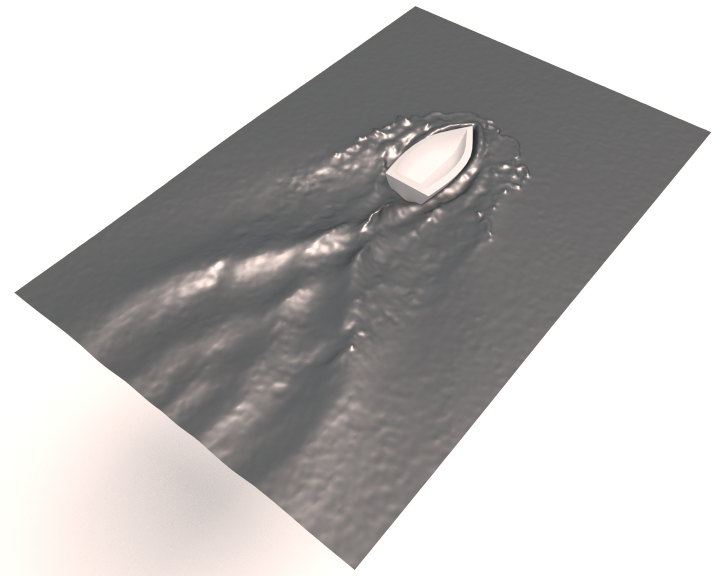
\includegraphics[width=\textwidth]{images/fluidsculpting-mig2016/results/boatTraversal.png}
		\caption{\label{fig:result_detail:boat}\scriptsize{Boat simulation}}
	\end{subfigure}
	\hspace{0.1cm}
	\begin{subfigure}[b]{0.40\linewidth}
		\centering
		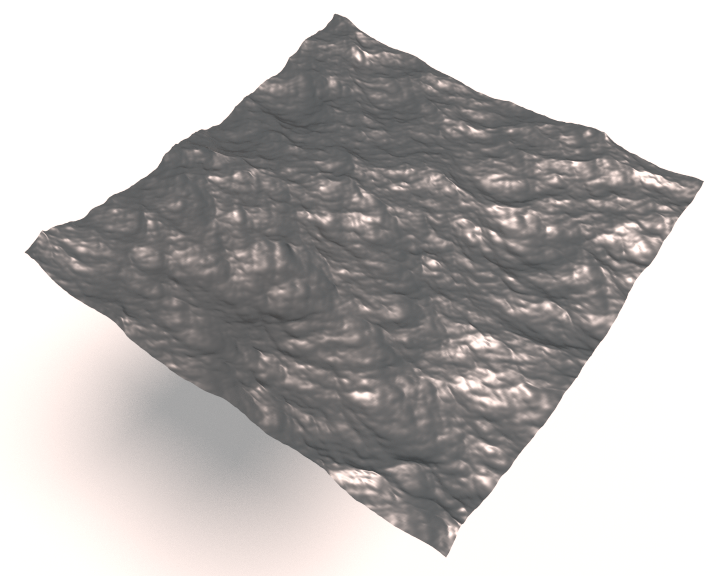
\includegraphics[width=\textwidth]{images/fluidsculpting-mig2016/results/highResOcean.png}
		\caption{\label{fig:result_detail:ocean}\scriptsize{Procedural ocean}}
	\end{subfigure}
	\hspace{0.1cm}
	\begin{subfigure}[b]{0.40\linewidth}
		\centering
		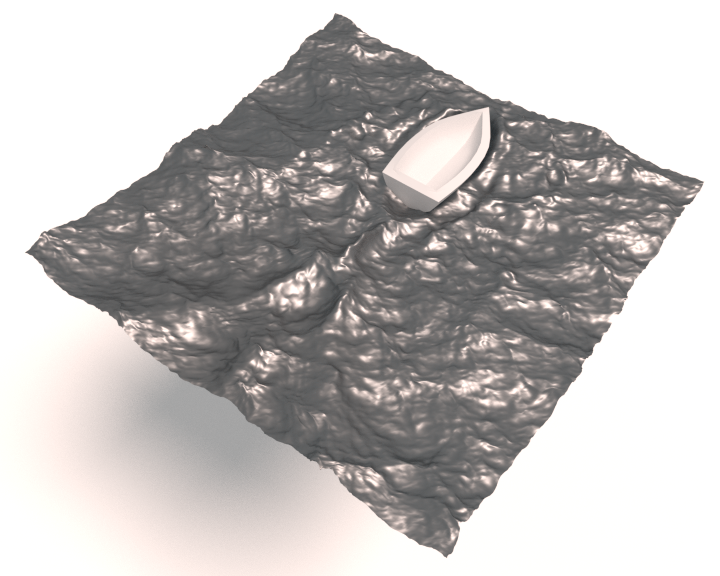
\includegraphics[width=\textwidth]{images/fluidsculpting-mig2016/results/boatOnOcean.png}
		\caption{\label{fig:result_detail:paste}\scriptsize{Pasting of the wake}}
	\end{subfigure}
	\hspace{0.1cm}
	\begin{subfigure}[b]{0.40\linewidth}
		\centering
		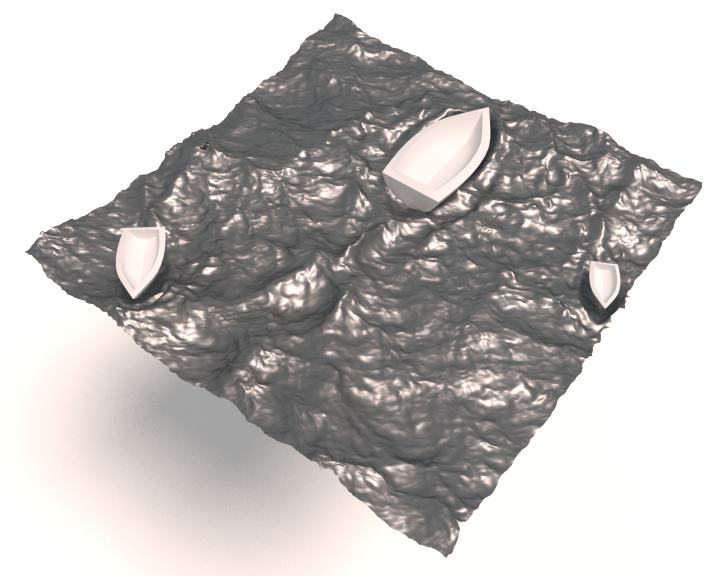
\includegraphics[width=\textwidth]{images/fluidsculpting-mig2016/results/threeBoatsOnOcean.png}
		\caption{\label{fig:result_detail:paste_2}\scriptsize{Multiple pasting}}
	\end{subfigure}
	\caption[Fluid sculpting: Boat wake]{\label{fig:result:boatWake}
		From the animation of boat generated using a FLIP simulation (left), our sculpting system allows to extract the wake of the boat in a single \emph{space-time feature}. Then we can manipulate this feature and paste it into an ocean animation generated procedurally (middle). Editing the feature and pasting it multiple times allows to interactively model a complex scene (right) without re-simulating.
	}
\end{figure}

\paragraph{Animation enrichment}
An interesting aspect of our method is that it can be used to enrich static objects or non-fluid objects with a fluid-like behavior. 
In Figure~\ref{fig:result:teaser}, we enriched a static object with a splash extracted from a liquid animation.
More generally, our method allows to combines results obtained with very different methods such as procedural animation, Eulerian and Lagrangian simulations, shallow water simulation, or artist-created animations.

\begin{figure}[!h]
	\centering
	\begin{subfigure}[b]{0.40\linewidth}
		\centering
		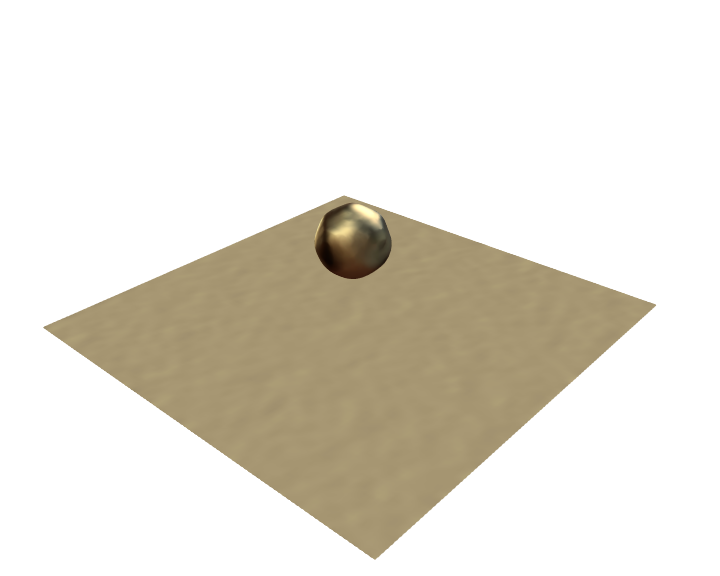
\includegraphics[width=\textwidth]{images/fluidsculpting-mig2016/teaser/fluid_004.png}
		\caption{\label{fig:result_detail:drop_0}\footnotesize{Initial simulation at time $t_0$}}
	\end{subfigure}
	\hspace{0.1cm}
	\begin{subfigure}[b]{0.40\linewidth}
		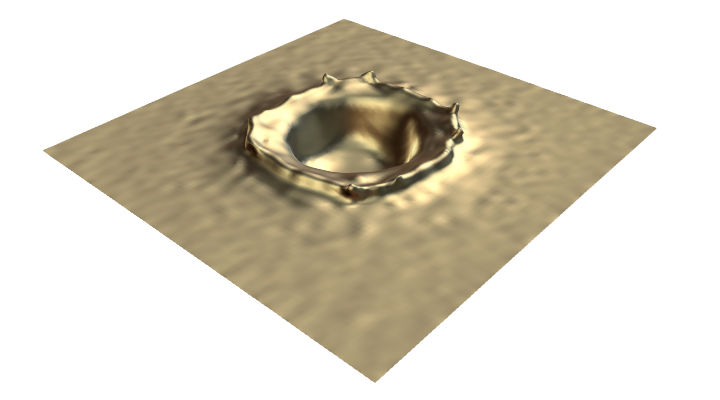
\includegraphics[width=\textwidth]{images/fluidsculpting-mig2016/teaser/fluid_012.png}
		\caption{\label{fig:result_detail:drop_1}\footnotesize{Initial simulation at time $t_1$}}
	\end{subfigure}
	\hspace{0.1cm}
	\begin{subfigure}[b]{0.40\linewidth}
		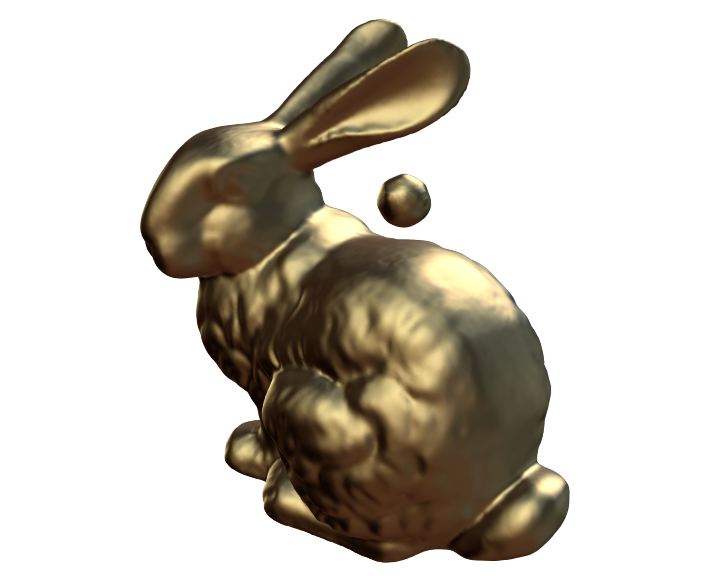
\includegraphics[width=\textwidth]{images/fluidsculpting-mig2016/teaser/bunny_04.png}
		\caption{\label{fig:result_detail:bunny_0}\footnotesize{Final animation at time $t_0$}}
	\end{subfigure}
	\hspace{0.1cm}
	\begin{subfigure}[b]{0.40\linewidth}
		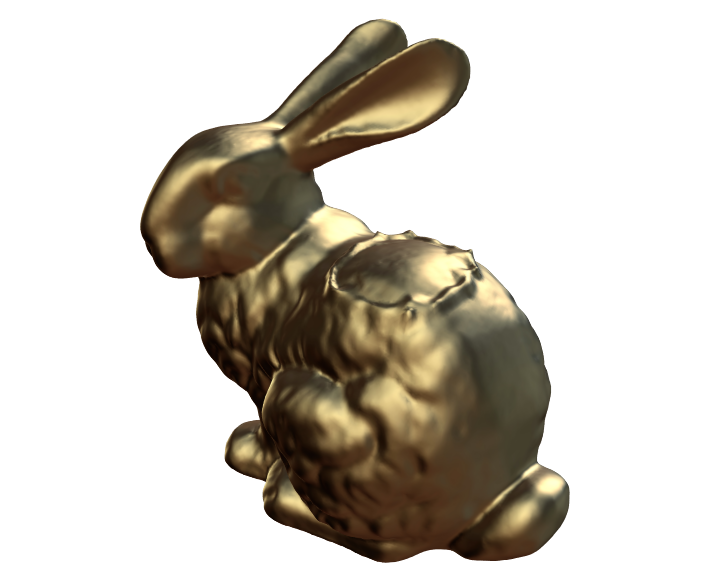
\includegraphics[width=\textwidth]{images/fluidsculpting-mig2016/teaser/bunny_12.png}
		\caption{\label{fig:result_detail:bunny_1}\footnotesize{Final animation at time $t_1$}}
	\end{subfigure}
	\caption[Fluid sculpting: Drop on bunny]{\label{fig:result:teaser}
		From an initial simulation of a falling drop (a, b) space-time features can be extracted and pasted back into an other mesh, generating a new animation (c, d).}
\end{figure}

\paragraph{Trajectory editing}

In Figure~\ref{fig:result_trajectory}, we applied several edits to a \emph{space-time feature} capturing a crown splash. First, we temporally remapped the feature to slow it down. 
Second, we pasted it twice on a static plane at different locations. 
Third, we edited the trajectory of the droplets to change the height of their fall. 
Finally, we used a fading out to obtain a smooth transition with the initial plane.

\begin{figure}[!h]
	\centering
	\begin{subfigure}[b]{0.3\linewidth}
		\centering
		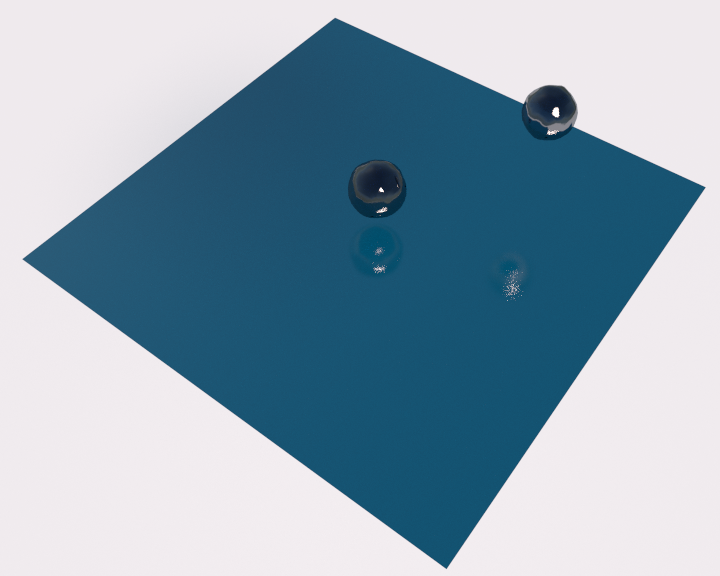
\includegraphics[width=\textwidth]{images/fluidsculpting-mig2016/results/two_drops_0.png}
		\caption{\label{fig:result_trajectory:t0}$t=t_{0}$}
	\end{subfigure}
	\hspace{0.1cm}
	\begin{subfigure}[b]{0.3\linewidth}
		\centering
		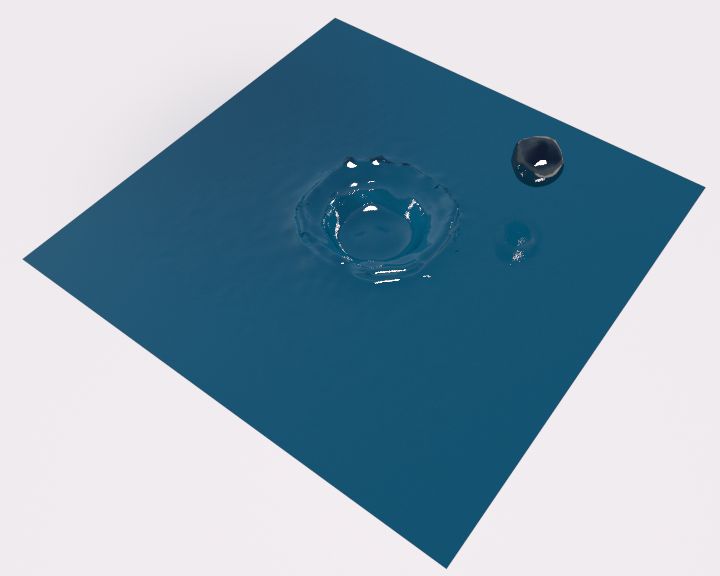
\includegraphics[width=\textwidth]{images/fluidsculpting-mig2016/results/two_drops_1.png}
		\caption{\label{fig:result_trajectory:t1}$t=t_{1}$}
	\end{subfigure}
	\hspace{0.1cm}
	\begin{subfigure}[b]{0.3\linewidth}
		\centering
		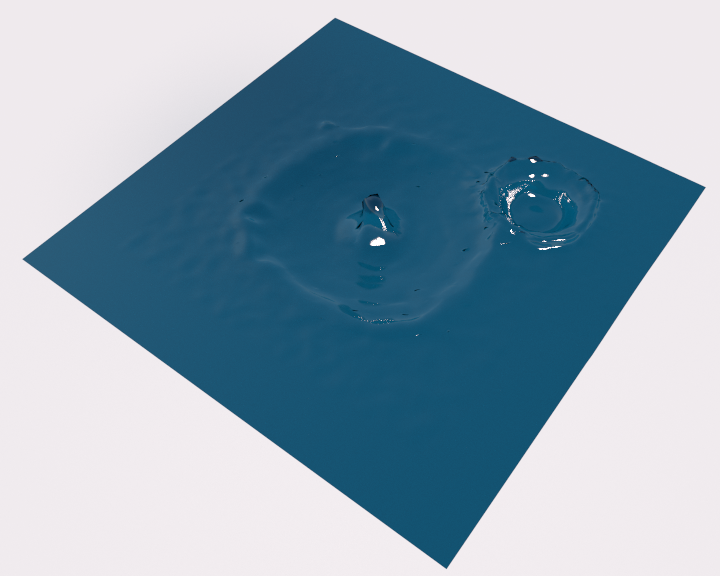
\includegraphics[width=\textwidth]{images/fluidsculpting-mig2016/results/two_drops_2.png}
		\caption{\label{fig:result_trajectory:t2}$t=t_{2}$}
	\end{subfigure}
	\caption[Fluid sculpting: Droplets]{From an existing liquid animation we extracted a complete crown splash into a single \emph{space-time feature}. The feature combines both the fall of a drop and the resulting splash. We edit and paste this feature twice at different locations and modify the height of the droplets. Here, we show different frames of the final animation.
	}
	\label{fig:result_trajectory}
\end{figure}

\newpage 

\section{Discussion and concluding remarks} \label{sec:fluidsculpting:discussion}

In this chapter, we introduced a new method for interactively editing existing fluid animations. We based our approach on an intuitive sculpting metaphor where the user can select, copy, edit and paste coherent \emph{space-time features}. 
This approach allows a user to quickly design new liquid animations. 
Our method is not without limitations, and we suggest several directions for future work.

\subparagraph{Physical consistency} 
Even though the space-time features selected by the user capture realistic behavior, the way they are edited and inserted may spoil the realism of the resulting animation. 
As we do not check for physical consistency, the plausibility of the result depends on the user's artistic skill. 
An extension of our method would be to adapt the destination surface so that it matches the input features under physical constraints such as volume preservation. 
To incorporate further physical constraints such as momentum conservation, using mesh sequences as input would not be sufficient anymore and additional information such as velocity would be required. 
Designing an interactive editing method given these constraints may be difficult to achieve.

\subparagraph{Resolution issues} 
Geometrical details may be lost when pasting a feature if the resolution of the target mesh sequence is too coarse. 
To remedy this limitation, we could add an automatic mesh refinement scheme such that the resolution of the target mesh always locally matches the resolution of details in the pasted feature.

\subparagraph{Aggregation robustness} 
The aggregation of regions of interest into space-time features is a key component of our approach. 
However, as it is based on geometrical similarities between two consecutive frames, it might fail if the time step between two frames is too large or if parts of the water body are moving too fast, such as in the case of dynamic splashes with lots of fast moving droplets. 
Even if it has not been an issue for our results, we would like to enforce the robustness of the aggregation step by adding a new metric which would measure the physical coherency between two regions of interest. 
This metric would take into account some inferred velocity for the region. It could also incorporate some cause and effect relationships; for example, a falling drop will cause waves. 

\subparagraph{Memory consumption} 
For our results, we worked with short sequence of liquid animations but when editing a large sequence of high resolution meshes and extracting potentially large space-time features, memory consumption may become a problem. 
A classical solution would be to use a multi-resolution approach.
The user would manipulate a low resolution version of the animation which would ensure interactivity. 
Then, the user's edits choice would be transferred to the high resolution version of the animation as an off-line post-process.

\subparagraph{Feature editing} 
We proposed basic tools for the space-time edition of features and there are several avenues for future work. 
Firstly, our copy/paste method is only able to deal with simple deformations of a surface. 
By using the work of~\cite{Takahashi2003} to extract and insert displacement fields, we could handle much more complex cases. 
Secondly, we would like to propose a space-time sculpting tool close to space deformers such as constant volume tools~\cite{Angelidis2006b,funk2006vector} and topology modifiers~\cite{stanculescu2011freestyle}. 
The idea would be to let the user sculpt a specific frame and to interpolate the deformation over time. 
Finally, we think it would be useful to let any edited parameter (scale, rotation, etc.) to be key-framed in order to make time-varying effects more easily controllable.
%In the future, we think that our representation for \emph{space-time features} could be extended and used to manipulate animations at a higher level, similarly to a story-board. 
%\newpage
%\appendix

%\section{Notation table}
%\label{sec:notations}
%
%\begin{table}[htbp]
%\centering
%\small
%    \begin{tabular}{ rl }
%        \hline
%        \textbf{Symbol}     & \textbf{Description} \\
%        \hline
%        $M = (M^t)_{0 \leq t < T(M)}$       & Mesh sequence \\
%        $T(.)$              & Number of frames in argument \\
%        $L(.)$              & Characteristic length in argument \\
%        $N_X$               & Nodes of mesh $X$ \\
%        $P_X$               & Polygonal faces of mesh $X$ \\
%        $pos(n, X)$         & Position of vertex $n\in N_X$ \\
%        $norm(n, X)$        & Normal of vertex $n\in N_X$ \\
%        $disp(n, X_1, X_2)$ & $pos(n, X_2) - pos(n, X_1)$ \\
%        \hline
%        $F_i = (F_i^t)_{t^s(F_i) \leq t \leq t^e(F_i)}$   & $i^{th}$ feature of the animation\\
%        $t^{s/e}(F_i)$      & Starting/ending frame index of $F_i$ \\
%        $S(F^t_i)$          & Part of $M^t$ corresponding to $F^t_i$ \\
%        $X'$                & Smoothed version of mesh or mesh part $X$ \\
%        $M(F^t_i)$          & Mesh representation of $F^t_i$\\
%        $(\tau_d(F^t_i), \tau_n(F^t_i))$ & Differential representation of $F^t_i$\\
%        $C(X)$              & Centre of mass of surface $X$ \\
%        $A(X)$              & Area of surface $X$ \\
%        $V(X)$              & Volume of surface $X$ \\
%        \hline
%        $G$                 & Frame features adjacency graph \\
%        $V_G = \{F_j^t\}_{t,j}$ & Vertices of graph $G$ \\
%        $E_G = \{e^t_{ij}\}_{t, r(i,j)}$ & Edges of graph $G$ \\
%        $\omega^t_{ij}$     & Cost of $e^t_{ij}$ (see Equation~\ref{eq:costfunction}) \\
%        $d^t_{ij}$          & $\|C(S(F^t_i)) - C(S(_j^{t+1}))\|$ \\
%        $a^t_{ij}$          & $\|A(S(F^t_i)) - A(S(_j^{t+1}))\|$ \\
%        $v^t_{ij}$          & $\|V(S(F^t_i)) - V(S(_j^{t+1}))\|$ \\
%        $\omega_d$          & Edge cost distance weight \\
%        $\omega_a$          & Edge cost area weight \\
%        $\omega_v$          & Edge cost volume weight \\
%        \hline
%    \end{tabular}
%\caption{Notations used throughout this article.
%Subscript (resp. superscript) indices are used for spatial (resp. temporal) indexing.
%Parenthesis (resp curly braces) are used for ordered (resp unordered) sets.}
%\label{tab:notation}
%\end{table}
%
%\section{Mesh part manipulation}
%\label{sec:mesh_part}
%
%We define $R$ a part of mesh $X=(N_X, P_X)$ as a subset of its vertices: $R\subset N_X$.
%$R$ being itself a set, usual set operations can be performed on it such as union, intersection and difference.
%
%The border of $R$, noted $\partial R$, is defined by:
%\begin{equation}
% \partial R = \{ n \in R \vert \exists n_i \in neib(n), n_i \not\in R \}
%\end{equation}
%where $neib(n)$ is the set of neighbors of $n$ in $X$:
%\begin{equation}
% neib(n) = \{ n' \in N_X \vert \exists p \in P_X, n \in p \cup n' \in p \} 
%\end{equation}
%
%\paragraph{Mathematical morphology operators.}
%$R$ can be \emph{eroded} into $ero(R)$ using the following relation:
%\begin{equation}
% ero(R) = \{ n \in R \vert \nexists n_i \in neib(n), n_i \not\in R \}
%\end{equation}
%which is equivalent to $ero(R) = R \setminus \partial R$.
%
%Reciprocally, $R$ can be \emph{dilated} into $dil(R)$ using the following relation:
%\begin{equation}
% dil(R) = \{ n \in N_X \vert \exists n_i \in neib(n), n_i \in R \}
%\end{equation}
%
%Dilation can be extended to an arbitrary order $k$:
%\begin{equation}
% dil^k(R) = \underbrace{dil(\dots dil(}_{\text{$k$ terms}}R)\dots)
%\end{equation}
%The same stands for erosion:
%\begin{equation}
% ero^k(R) = \underbrace{ero(\dots ero(}_{\text{$k$ terms}}R)\dots)
%\end{equation}
%
%We call \emph{opening} of order $k$ the mesh part defined as:
%\begin{equation}
% ope^k(R) = dil^k(ero^k(R))
%\end{equation}
%and \emph{closure} of order $k$ the mesh part defined as:
%\begin{equation}
% clo^k(R) = ero^k(dil^k(R))
%\end{equation}
